\chapter{Realizace}
Popis implementace/realizace se zaměřením na nestandardní části řešení.

\section{Průběh realizace}
Fáze 1 
Po analýze a návrhu byla naimplementována zkušební část, kvůli ověření návrhu tříd a rozhraní. Na této verzi byla napsáno první velká část unit testů. Verze ukládala pouze do instancí nebo polí.
Fáze 2
Zprovoznění komunikace s databází. Hledání alternativních možností(sedna apod). Napsání eXistAPI.
Fáze 3
Předělání první verze implementace RubyACL z polové/instanční na databázovou. Přepsání tříd z instančních na jakési singlotonské managery. Všechny informace jsou uloženy v databázi. RubyACl pouze vkládá nové záznamy, upravuje a maže staré. Na existujících provádí dotazy a rozhodování o přístupu.
Fáze 4
Návrh tříd byl trochu chybný. Implementace předchozích verzí se odchylovala návrhu. Předělání tříd. Vytvoření nadřazené třídy ACL\_Object a dědění z této třídy. Intenzivní testování. Usnadnilo odhalit spousty chyb.
Fáze 5
Dokončení rozhodovací metody. Dotahování funkcionality. Opravování chyb a nedostatků. Testování v této fázi nejintenzivnější. Dokumentace.
Fáze 6
Finalizování - rakefile, rubygem. Dokumentace


\section{Programy použité při vývoji}
\begin{itemize}
\item NetBeans s Ruby platformou od Thomase Enebo
http://blog.enebo.com/
http://plugins.netbeans.org/plugin/38549/ruby-and-rails
\item GIT
https://github.com/sirljan/Ruby-ACL
\item eXist-db
http://www.exist-db.org
\item Enterprise Architect
\item MikTex
\end{itemize}
%-------------------------------------
\section{Databáze}
Protože XML databáze, která má RubyACL používat, není plně funkční, nebylo možné implementaci testovat přímo na ní. Za tímto učelem se musela vybrat jiná podobná databáze.

\subsection{Sedna}
Sedna knihovna v Ruby poskytuje rozhraní pro databázi Sedna. Klient je Ruby rozšíření, které používá ovladač jazyka C, který je dodáván jako součást distribuce Sedna. To má být jednoduché a snadno použitelné. Ovšem zprovoznění knihovny Sedna neproběhlo tak hladce, jak se tvrdí.

\subsection{eXist-db}
eXist-db je open source systém pro správu databáze vytvořena pomocí technologie XML. Ukládá XML data podle datového modelu XML a nabízí efektivní a XQuery zpracování založené na indexování. Podporuje velké množství technologií. Uvedu zde pouze ty, které se týkají RubyACL nebo eXistAPI: XPath 2.0(odkaz), XQuery(odkaz), XML-RPC(odkaz), XQuery Update Facility 1.0(odkaz). ExistAPI je komunikační rozhraní, které jsem byl nucený naimplementovat k lazení a testování RubyACL na eXist-db.

eXist-db se podobá XML databázi, která má RubyACL používat, a byla doporučena vedoucím práce jako ideální. Přesto proběhly komplikace s XUpdate navzdory přesné interpretace dokumentace. Z tohoto důvodu bylo nutné přejít na xQuery Update Facility


\subsubsection{eXistAPI}

Trochu nestandartní část realizace. Bylo potřeba si vytvořit komunikační rozhraní mezi databázi eXist-db a RubyACL.
ExistAPI je komunikační rozhraní, které bylo potřeba naimplementovat k ladění a testování RubyACL na eXist-db.
Komunikace s db pomocí eXistAPI.
Použití xQuery Update Facility místo xUpdate. (Možná vložím ukázku implementace)
Komunikace založená na protokolu XML-RPC. K dotazování využívá technologie xQuery a xPath. xQuery Update Facility je zapotřebí k editování dat v databázi.
TODO předělat v obrázku api na eXistAPI
\begin{figure}
%\centering
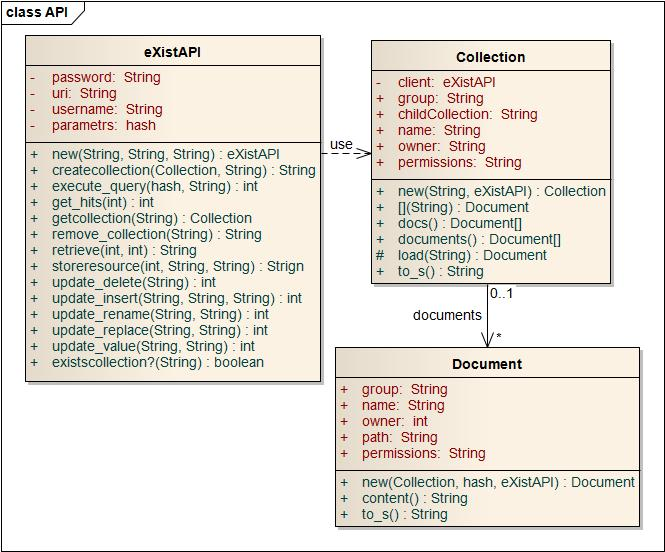
\includegraphics[width=15cm]{eXistAPI.jpg}
\caption{Diagram tříd TODO}
\label{fig:Diagram tříd TODO}
\end{figure}

%-------------------------------------
\section{Implementace}


%-------------------------------------

\subsection{pracovni poznamky}
\begin{itemize}
\item Je třeba se věnovat uvolňování paměti, protože aplikace bude spuštěna dny až měsíce. Špatné zacházení s pamětí by, proto bylo kritické pro server, na kterém aplikace s Ruby-ACL knihovnou bude spuštěna.
\item Ušetření času db serveru vhodným uspořádáním dotazů. Místo iterace dotazů jeden dotaz s vhodnou podmínkou. (tvoreni clenstvi) 
\item Pro identifikaci a propojení jsem uvažoval mezi xLink a idref. Idref nabízí jednoduchý systém, ale xLink nabídl podrobné specifikace W3C, velké množství návodů a turtoriálů a především se jedná o novější technologii, jejíž osvojení jsem považoval za výhodné. Rozhodl jsem se proto implementovat xLink. Problém nastal při některých vkládání textů a dotazování. EXist DB měla problém s jmeným prostorem xLink i přes zkutečnost, že jmený prostor byl uveden. Troufám si říct, že byl uveden správně, protože při většině použití fungoval. Než abych se zabýval mnoho času proč použití xLink nejde, raději jsem přešel na jednoduchý idref. Implementace idref proběhla bez problémů.
\item Občas je kód zdvojený, ale má to svoje opodstatnění. Například addmembership a addmembershippriv. Kdyby nebylo zdvojeno, šlo by přidávat privilige k principal a naopak.
\item predelavam structuru z tridniho volani na singleton nebo jak se to jmenuje.\item predelavam structuru z tridniho volani na singleton nebo jak se to jmenuje.
\item kdyz smazu nadrazenou skupinu tak smazu vsechny jeji clenstvi
\end{itemize}

\section{Zdrojové soubory}
zdrojové soubory jsou v xml formátu. Jejich strukturu popisují dtd soubory.